%++++++% Preâmbulo %+++++++++++++++++++++++++++++++++++++++++++++++++++++++++
\documentclass[13pt, xcolor={dvipsnames,svgnames}, portuguese]{beamer}
%\documentclass[[11pt, xcolor={dvipsnames,svgnames,table},portuguese]{beamer} 

\usetheme{CambridgeUS}

\setbeamercolor*{structure}{bg=PineGreen!20,fg=PineGreen} %fg=PineGreen
\definecolor{beamer@pinegreen}{rgb}{0.137,0.666,0.741}


\setbeamercolor*{palette primary}{use=structure,fg=white,bg=structure.fg}
\setbeamercolor*{palette secondary}{use=structure,fg=white,bg=structure.fg!75}
\setbeamercolor*{palette tertiary}{use=structure,fg=white,bg=structure.fg!50!black}
\setbeamercolor*{palette quaternary}{fg=white,bg=black}

\setbeamercolor{section in toc}{fg=black,bg=white}
\setbeamercolor{alerted text}{use=structure,fg=structure.fg!50!black!80!black}

\setbeamercolor{titlelike}{parent=palette primary,fg=structure.fg!50!black}
\setbeamercolor{frametitle}{bg=gray!10!white,fg=PineGreen}

\setbeamercolor*{titlelike}{parent=palette primary}

\usepackage[utf8]{inputenc}
\usepackage[brazil]{babel}  % idioma
\usepackage{amsmath,amsfonts,amssymb,textcomp}
\usepackage{graphicx}
\usepackage{subfigure}
\usepackage[utf8]{inputenc}
\usepackage{ifpdf}
\usepackage{listings}

% Configurações para o ambiente lstlisting
\lstset{
    language=C,
    basicstyle=\ttfamily\footnotesize,
    numbers=left,
    numberstyle=\tiny,
    numbersep=5pt
}

% here you should include other packages with \usepackage

    \ifpdf

      % hyperref should be the last package loaded:
	  %\usepackage[pdftex]{hyperref}
      \usepackage{pst-pdf}
    \else

      % make the command \href from hyperref available as a 'print only'
      \newcommand{\href}[2]{#2}

    \fi

%Global Background must be put in preamble
\usebackgroundtemplate%
{%
    
\includegraphics[width=\paperwidth,height=\paperheight]{Figuras/fundo.png}%
}
\setbeamertemplate{frametitle}[default][center]
 
\author{Othon Oliveira}
\title{Lógica de Programação com Java Script}
\institute{SENAC - PROA} 
\date{} 
%\subject{} 

\begin{document}

\begin{frame}
\titlepage
%\date{}
\end{frame}

% Capa - requer o TikZ
\newcommand{\capa}{
    \begin{tikzpicture}[remember picture,overlay]
        \node at (current page.south west)
            {\begin{tikzpicture}[remember picture, overlay]
                \fill[shading=radial,top color=orange,bottom color=orange,middle color=yellow] (0,0) rectangle (\paperwidth,\paperheight);
            \end{tikzpicture}
          };
    \end{tikzpicture}
}

\begin{frame}\frametitle{Sumário}
\tableofcontents
\end{frame}


%+++++++++++++++++++++++++++++++++++++++++++++++
\section{Entrutura das páginas do seu projeto}
%+++++++++++++++++++++++++++++++++++++++++++++++
\begin{frame}{Introdução a Lógica de Programação com Java Script}
\framesubtitle{ Locais quase obrigatírios do Java Script/CSS}
	\begin{block}{Com organizar seu código}
		\begin{itemize}
		  \item[a.] O Java Script deve ficar num arquivo separado do HTML
		  \pause
		  \item[b.] Normalmente um ``seu\_arquivo.js'' fica numa pasta separada
		   \pause		  
		  \item[c.] O arquivo CSS também segue a mesma lógica anterior
		  \pause
		  \item[d.] Dessa forma, seu código ficará organizado e fácil de ser encontrado
		\end{itemize}
	\end{block} 
\end{frame}

%+++++++++++++++++++++++++++++++++++++++++++++++
\section{Como fica seu projeto: sugestão}
%+++++++++++++++++++++++++++++++++++++++++++++++

\begin{frame}[fragile]
\frametitle{Exemplo de arquivo.css}
\framesubtitle{Nome do aquivo: style.css}

\begin{verbatim}
/* style.css */

body {
  font-family: Arial, sans-serif;
  background-color: #f0f0f0;
}

h1 {  color: blue; }

p {  font-size: 16px;
  margin-bottom: 10px;
}

\end{verbatim}
\end{frame}
%-------------------------------------------------------------
\begin{frame}[fragile]

\begin{verbatim}
<!DOCTYPE html>
<html>
<head>
  <title>Exemplo de CSS com arquivo separado</title>
  <link rel="stylesheet" type="text/css" href="style.css">
</head>
<body>
  <h1>Título da Página</h1>
  <p>Este é um parágrafo com estilo definido.</p>
</body>
</html>
\end{verbatim}
Vincular é o mesmo que "conectar, ligar,.."

\end{frame}

%+++++++++++++++++++++++++++++++++++++++++++++++
\section{Estrutura raiz do projeto}
%+++++++++++++++++++++++++++++++++++++++++++++++
\begin{frame}
\frametitle{Apresentando o seu projeto}

Seu projeto ficará, mais ou menos assim:
\begin{figure}
  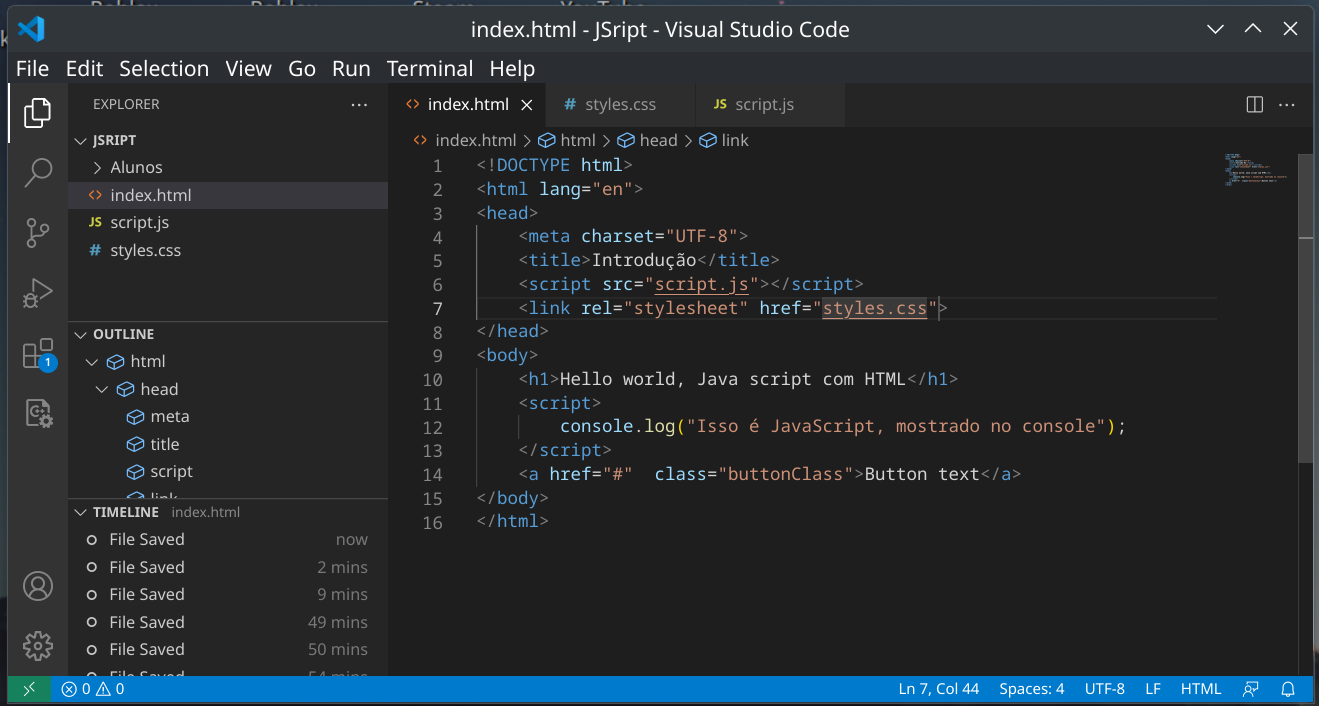
\includegraphics[width=0.85\textwidth]{Figuras/estruturaSite.png}
  \caption{Estrutura do projeto}
\end{figure}
A página ``index.html'' geralemente é mandatória pelos servidores Web
\end{frame}

%+++++++++++++++++++++++++++++++++++++++++++++++++++++++++++++
\section{Estruturas de repetição em JavaScript}
%+++++++++++++++++++++++++++++++++++++++++++++++++++++++++++++

\begin{frame}[fragile]
\frametitle{Estruturas de Repetição em JavaScript}

\textbf{Estrutura "for"}

\begin{verbatim}
for (inicialização; condição; atualização) {
  // Código a ser executado
}
\end{verbatim}

\begin{itemize}
  \item Inicialização: Define o valor inicial da variável de controle.
  \item Condição: Verifica se a repetição deve continuar.
  \item Atualização: Atualiza a variável de controle após cada iteração.
\end{itemize}

\end{frame}
%-------------------------------------------------------------------
\begin{frame}[fragile]
\frametitle{Estruturas de Repetição em JavaScript}

\textbf{Estrutura "while"}

\begin{verbatim}
while (condição) {
  // Código a ser executado
}
\end{verbatim}

\begin{itemize}
  \item A repetição ocorre enquanto a condição for verdadeira.
  \item A condição é verificada antes de cada iteração.
  \item Certifique-se de que a condição seja eventualmente falsa para evitar loops infinitos.
\end{itemize}

\end{frame}


%-------------------------------------------------------------------
\begin{frame}[fragile]
\frametitle{Estruturas de Repetição em JavaScript}

\textbf{Estrutura "do-while"}

\begin{verbatim}
do {
  // Código a ser executado
} while (condição);
\end{verbatim}

\begin{itemize}
  \item A repetição ocorre pelo menos uma vez, pois a condição é verificada após a execução do bloco.
  \item O código é executado primeiro e a condição é verificada depois.
  \item A condição determina se o loop continua ou não.
\end{itemize}

\end{frame}

%------------------------------------------------------

\begin{frame}[fragile]
\frametitle{Estruturas de Repetição especiais em JavaScript}

\textbf{Loop For...in}

\begin{verbatim}
const person = { name: "John", age: 30 };
for (let key in person) {
  console.log(key + ": " + person[key]);
}
\end{verbatim}

\begin{itemize}
  \item O loop "for...in" itera sobre as propriedades de um objeto.
  \item Em cada iteração, a variável "key" contém o nome da propriedade.
  \item Pode ser útil para percorrer propriedades de objetos ou elementos de um array associativo.
\end{itemize}

\end{frame}

\begin{frame}[fragile]
\frametitle{Estruturas de Repetição especiais em JavaScript}

\textbf{Loop For...of}

\begin{verbatim}
const numeros = [1, 2, 3, 4, 5];
for (let num of numeros) {
  console.log(num);
}
\end{verbatim}

\begin{itemize}
  \item O loop "for...of" itera sobre os valores de um objeto iterável, como um array.
  \item Em cada iteração, a variável "num" contém o valor do elemento atual.
  \item É uma forma mais simples de percorrer os elementos de um array.
\end{itemize}

\end{frame}

%++++++++++++++++++++++++++++++++++++++++++++++++++
\subsection{Sobre o uso de variáveis em JavaScript}
%++++++++++++++++++++++++++++++++++++++++++++++++++

\begin{frame}[fragile]
\frametitle{Declaração de Variáveis em JavaScript}

\textbf{let vs. var vs. const}

\begin{itemize}
  \item \textbf{let}: Introduz uma variável de escopo de bloco.
  \item \textbf{var}: Introduz uma variável de escopo de função ou global.
  \item \textbf{const}: Introduz uma constante de escopo de bloco.
\end{itemize}

\begin{verbatim}
// Exemplos:
let x = 10;        // Escopo de bloco
var y = 20;        // Escopo de função/global
const z = 30;      // Constante de bloco
\end{verbatim}

\begin{itemize}
  \item Use `let` para criar variáveis com escopo mais restrito.
  \item Use `var` com cautela, devido ao seu escopo menos restrito.
  \item Use `const` para criar constantes imutáveis.
\end{itemize}

\end{frame}
%-------------------------------------------
\begin{frame}[fragile]
\frametitle{Declaração de Variáveis em JavaScript}

\textbf{Problemas do uso de let e var}

\textbf{Problemas com "var":}

\begin{itemize}
  \item Escopo global ou de função pode causar bugs.
  \item Hoisting pode levar a comportamentos inesperados.
\end{itemize}

\textbf{Problemas com "let":}

\begin{itemize}
  \item Escopo de bloco mais restrito ajuda a evitar bugs.
  \item Variáveis declaradas com "let" não são hoisted.
  \item Uso em loops pode causar problemas de closure.
\end{itemize}

\textbf{Recomendação:}

\begin{itemize}
  \item Prefira usar "let" para evitar bugs de escopo e hoisting.
  \item Evite o uso de "var" para declarações de variáveis.
\end{itemize}

\end{frame}
%-------------------------------------------

\begin{frame}[fragile]
\frametitle{Hoisting em JavaScript}

\textbf{Hoisting}

\begin{itemize}
  \item Hoisting é o comportamento em que declarações de variáveis e funções são movidas para o topo de seu escopo antes da execução do código.
  \item Isso significa que você pode usar variáveis antes de declará-las.
\end{itemize}

\textbf{Exemplo de Hoisting com "var":}

\begin{verbatim}
console.log(x); // variável indefinida ainda
var x = 10;     // variável definia e atribuída
\end{verbatim}

\textbf{Exemplo de Hoisting com "let" e "const":}

\begin{verbatim}
console.log(y); // ReferenceError (erro de referência
let y = 20;
\end{verbatim}

\textbf{Dica:}

\begin{itemize}
  \item Evite hoisting não intencional usando "let" e "const".
\end{itemize}

\end{frame}

%+++++++++++++++++++++++++++++++++++++++++++
\subsection{Vendo exemplos práticos}
%+++++++++++++++++++++++++++++++++++++++++++
\begin{frame}[fragile]
\frametitle{Estruturas de Repetição em JavaScript}

\textbf{1. Laço (ou loop)- For}

\begin{verbatim}
for (let i = 0; i < 5; i++) {
  console.log(i);
}
\end{verbatim}

\end{frame}
%-------------------------------------------------------------
\begin{frame}[fragile]
\frametitle{Estruturas de Repetição em JavaScript}

\textbf{2. Laço (ou loop)- While}

\begin{verbatim}
let counter = 0;
while (counter < 5) {
  console.log(counter);
  counter++;
}
\end{verbatim}

\end{frame}
%-------------------------------------------------------------
\begin{frame}[fragile]
\frametitle{Estruturas de Repetição em JavaScript}

\textbf{3. Laço (ou loop)- \"Do While\"}

\begin{verbatim}
let number = 1;
do {
  console.log(number);
  number++;
} while (number <= 5);
\end{verbatim}

\end{frame}
%-------------------------------------------------------------
\begin{frame}[fragile]
\frametitle{Estruturas de Repetição em JavaScript}

\textbf{Usando o Break para sair da repetição }

\begin{verbatim}
for (let i = 0; i < 10; i++) {
  if (i === 5) {
    break;
  }
  console.log(i);
}
\end{verbatim}

\end{frame}
%-------------------------------------------------------------
\begin{frame}[fragile]
\frametitle{Estruturas de Repetição em JavaScript}

\textbf{5. O comando: Continue}

\begin{verbatim}
for (let i = 0; i < 5; i++) {
  if (i === 2) {
    continue;
  }
  console.log(i);
}
\end{verbatim}

\end{frame}
%-------------------------------------------------------------
\begin{frame}[fragile]
\frametitle{Estruturas de Repetição em JavaScript}

\textbf{6. Laço (ou loop)- For...in}

\begin{verbatim}
const pessoas = { nome: "John", idade: 30 };
for (let chave in pessoas) {
  console.log(key + ": " + pessoas[chave]);
}
\end{verbatim}

\end{frame}
%-------------------------------------------------------------
\begin{frame}[fragile]
\frametitle{Estruturas de Repetição em JavaScript}

\textbf{7. Laço (ou loop)- For...of}

\begin{verbatim}
const numbers = [1, 2, 3, 4, 5];
for (let num of numbers) {
  console.log(num);
}
\end{verbatim}

\end{frame}
%-------------------------------------------------------------
\begin{frame}[fragile]
\frametitle{Estruturas de Repetição em JavaScript}

\textbf{8. Laços (loops) aninhados}

\begin{verbatim}
for (let i = 0; i < 3; i++) {
  for (let j = 0; j < 2; j++) {
    console.log(i, j);
  }
}
\end{verbatim}

\end{frame}
%-------------------------------------------------------------
\begin{frame}[fragile]
\frametitle{Estruturas de Repetição em JavaScript}

\textbf{9. laço While com Break}

\begin{verbatim}
let num = 1;
while (true) {
  console.log(num);
  num++;
  if (num > 5) {
    break;
  }
}
\end{verbatim}

\end{frame}
%-------------------------------------------------------------
\begin{frame}[fragile]
\frametitle{Estruturas de Repetição em JavaScript}

\textbf{10. laço While com Continue}

\begin{verbatim}
let num = 0;
while (num < 5) {
  num++;
  if (num === 3) {
    continue;
  }
  console.log(num);
}
\end{verbatim}

\end{frame}

%-------------------------------------------------------------
\section{Teste de primalidade}
\subsection{Vários tipos de algoritmos para testar se é primo}
%-------------------------------------------------------------
\begin{frame}[fragile]
\frametitle{Teste de números primos - primalidade}
Função para verificar se um número é primo
\begin{verbatim}
function ehPrimo(numero) {
  if (numero <= 1) { return false; }
  if (numero <= 3) { return true;  }
  if (numero % 2 === 0 || numero % 3 === 0) {
    return false;
  }
  for (let i = 5; i * i <= number; i += 6) {
    if (number % i === 0 || number % (i + 2) === 0) {
      return false;
    }
  }
  return true;
}
\end{verbatim}
\end{frame}


%%+++++++++++++++++++++++++++++++++++++++++++++++


%+++++++++++++++++++++++++++++++++++++++++++++++




%-----------------------------------------------

\end{document}